%%%%%%%%%%%%%%%%%%%%%%%%%%%%%%%%%%%%%%%%%
% Šablona pro závěrečné práce na UPCE
% Verse 1.0 (2018/10/29)
%
% Autor:
% Petr Vnenk (petr.vnenk@student.upce.cz)
%
% Licence:
% CC-BY
%
%%%%%%%%%%%%%%%%%%%%%%%%%%%%%%%%%%%%%%%%%

%------------------------------------------
% ÚVODNÍ DEFINICE A SEZNAM BALÍČKŮ; v prvním řádku nastaveno "cs_CZ" pro kontrolu českého pravopisu
%------------------------------------------

% !TeX spellcheck = cs_CZ
\documentclass[12pt,a4paper]{report}															% základní velikost písma, formát papíru

\usepackage[english,czech]{babel}																% jazykový balíček
\usepackage[utf8]{inputenc}																		% kódování textu
\usepackage{graphicx}																			% zahrnutí různých grafických prvků
\graphicspath{{figures/}}																		% cesta ke složce s obrázky použitými v práci - vložte vlastní!
\usepackage{textcomp}																			% použití různých grafických symbolů
\usepackage[unicode]{hyperref}																	% tvorba hypertextových odkazů
\usepackage{array}																				% tvorba polí a tabulek
\usepackage{tabu}																				% tvorba komplikovanějších a dlouhých tabulek
\usepackage{gensymb}																			% balíček dalších užitečných symbolů
\usepackage{float}																				% práce s plovoucími objekty
\usepackage[top=2.5cm, left=3.5cm, right=1.5cm, bottom=2.5cm]{geometry}							% nastavení velikosti okrajů stránky
\usepackage{titlesec}																			% přenastavení parametrů nadpisů
\usepackage[hang,flushmargin]{footmisc}															% nastavení parametrů poznámek pod čarou
\usepackage[labelfont=bf, labelsep=endash]{caption}												% úprava nadpisů tabulek a popisů obrázků
\usepackage[nottoc]{tocbibind}																	% automaticky přidá seznam literatury, rejstřík a obsah do obsahu
\usepackage{url}																				% zajišťuje správnou funkčnost hypertextových odkazů
\usepackage{setspace}																			% nastavení rozestupu mezi řádky dokumentu
\usepackage{amsmath}																			% rozšířené použití matematických výrazů
\usepackage{booktabs}																			% rozšířené možnosti úprav tabulek
\usepackage{multirow}																			% obsah buňek tabulky přes více řádků
\usepackage{graphics}																			% základní balíček pro práci s grafikou
\usepackage[
backend=biber																					% nastavte biber místo BibTexu do kompilátoru!
,style=iso-numeric
,sortlocale=cs_CZ
,autolang=other
,bibencoding=UTF8
]{biblatex}																						% rozšířené možnosti práce s bibliografií
\addbibresource{literatura.bib}																	% zdrojové soubory literatury - vložte vlastní!
\usepackage[table]{xcolor}																		% práce s barvami
\usepackage{csquotes}																			% rozšířená práce s uvozovkami
\setlength{\arrayrulewidth}{0.5mm}																% nastavení tloušťky čar tabulky
\setstretch{1.242}																				% nastavení řádkování
\setlength{\parskip}{1em}																		% rozestup sousedních odstavců
\setlength\parindent{0pt}																		% odsazení prvního řádku odstavce
\titleformat{\chapter}{\bfseries\fontsize{17.28pt}{21pt}\selectfont}{\thechapter}{0.5em}{}		% formát nadpisů 1. řádu
\titleformat{\section}{\bfseries\fontsize{14pt}{17pt}\selectfont}{\thesection}{0.5em}{}			% formát nadpisů 2. řádu
\titleformat{\subsection}{\bfseries\fontsize{12pt}{14pt}\selectfont}{\thesubsection}{0.5em}{}	% formát nadpisů 3. řádu

\begin{document}

%------------------------------------------
% TITULNÍ LIST
%------------------------------------------

\begin{center}
{
\fontsize{14pt}{21pt}\selectfont																% velikost písma názvu university a fakulty
Univerzita Pardubice \\																			% název university 
\vspace{10pt}																					% vertikální mezera
Dopravní fakulta Jana Pernera \\																% název fakulty
\vspace{250pt}																					% vertikální mezera
\fontsize{14pt}{21pt}\selectfont																% velikost písma názvu práce
Název práce \\																					% název práce
\vspace{10pt}																					% vertikální mezera
\fontsize{14pt}{21pt}\selectfont																% velikost písma jména autora
Jméno Příjmení \\																				% jméno autora
\vspace{250pt}																					% vertikální mezera
Bakalářská práce \\																				% typ práce (bakalářská, diplomová, ...)
\vspace{10pt}																					% vertikální mezera
2018																							% rok publikace
}
\end{center}
\thispagestyle{empty}
\newpage

%------------------------------------------
% ZADÁNÍ PRÁCE
%------------------------------------------

Zadání -- první strana
\thispagestyle{empty}
\newpage

Zadání -- druhá strana
\thispagestyle{empty}
\newpage

%------------------------------------------
% PROHLÁŠENÍ AUTORA
%------------------------------------------

\vspace*{100pt}																					% vertikální mezera
Prohlašuji:

Tuto práci jsem vypracoval samostatně. Veškeré literární prameny a~informace, které jsem v~práci využil, jsou uvedeny v seznamu použité literatury.

Byl jsem seznámen s~tím, že se na moji práci vztahují práva a~povinnosti vyplývající ze zákona č.~121/2000 Sb., autorský zákon, zejména se skutečností, že Univerzita Pardubice má právo na uzavření licenční smlouvy o~užití této práce jako školního díla podle §~60 odst.~1 autorského zákona, a~s~tím, že pokud dojde k~užití této práce mnou nebo bude poskytnuta licence o~užití jinému subjektu, je Univerzita Pardubice oprávněna ode mne požadovat přiměřený příspěvek na úhradu nákladů, které na vytvoření díla vynaložila, a~to podle okolností až do jejich skutečné výše.

Beru na vědomí, že v~souladu s~§~47b zákona č.~111/1998 Sb., o~vysokých školách a~o~změně a~doplnění dalších zákonů (zákon o~vysokých školách), ve znění pozdějších předpisů, a~směrnicí Univerzity Pardubice č.~9/2012, bude práce zveřejněna v~Univerzitní knihovně a~prostřednictvím Digitální knihovny Univerzity Pardubice.

Tato diplomová práce byla realizována s~využitím technologií Výukového a~výzkumného centra v~dopravě.

\vspace*{84pt}
V~Pardubicích, dne 1. ledna 2018																% místo a datum

\vspace*{84pt}
\hspace*{300pt}																					% horizontální mezera
Jméno Příjmení

\thispagestyle{empty}
\newpage

%------------------------------------------
% PODĚKOVÁNÍ
%------------------------------------------

Rád bych poděkoval tomu, tomu a tamtomu též.													% poděkování
\thispagestyle{empty}
\newpage

%------------------------------------------
% ANOTACE A KLÍČOVÁ SLOVA
%------------------------------------------

\section*{Anotace}
Stručný obsah práce ve 3-4 větách, zapsaný v jazyce práce.										% anotace

\textbf{Příklad:} \textit{Práce je věnována stručným dějinám tělovýchovy a~sportu se zaměřením na jejich ženská odvětví a~stručnému vývoji dámského odívání se zaměřením na sportovní oblečení. Postihuje období od druhé poloviny 19.~století do druhé světové války a~zahrnuje území střední Evropy se zaměřením na České země. Zabývá se vlivem sportu na ženské odívání z~hlediska jeho vývoje v~uvedeném časovém období.}

\section*{Klíčová slova}
4-6 slov přesně vystihujících obsah práce, zapisují se s~malým počátečním písmenem, zpravidla jsou uvedena v~množném čísle. Nepoužívají se obecné (nadbytečné) termíny, znaky a~zkratky („např.“, „aj.“, „…“, „apod.“,…).										% klíčová slova

\textbf{Příklad:} \textit{sport, móda, ženy, odívání, 19.-20.~století}

\section*{Title}
Překlad názvu do angličtiny.																	% název v AJ

\section*{Annotation}
Překlad anotace do angličtiny.																	% anotace v AJ

\section*{Keywords}
Překlad klíčových slov do angličtiny.															% klíčová slova v AJ
\thispagestyle{empty}

%------------------------------------------
% OBSAH PRÁCE
%------------------------------------------

\tableofcontents
%\thispagestyle{empty}

%------------------------------------------
% SEZNAMY OBRÁZKŮ, TABULEK, ZKRATEK A TERMINOLOGIE
%------------------------------------------

\listoffigures
%\thispagestyle{empty}

\listoftables
%\thispagestyle{empty}

\chapter*{Seznam zkratek}
\addcontentsline{toc}{chapter}{Seznam zkratek}													% název do obsahu
\textit{V~abecedním pořadí:}

\begin{tabular}{ p{2cm} p{0.5cm} p{12cm} }
DÚ & -- & Drážní úřad\\ [1.242ex]																% položky seznamu zkratek
SŽDC & -- & Správa železniční dopravní cesty\\ [1.242ex]
\end{tabular}
%\thispagestyle{empty}

\chapter*{Terminologie}
\addcontentsline{toc}{chapter}{Terminologie}													% název do obsahu
\textit{Informační gramotnost:} schopnost jednotlivce prostřednictvím dostupných informačních metod a~technologií vyhledávat, zpracovávat, vyhodnocovat a~využívat informace.
\thispagestyle{empty}

%------------------------------------------
% VLASTNÍ TEXT PRÁCE
%------------------------------------------

\chapter{Úvod}

V~této šabloně jsou uplatněny jak všechny povinné prvky podle znění Směrnice Univerzity Pardubice č.~9/2012 ve znění platném k~datu vydání této verse šablony, tak také většina ostatních (doporučených). Několik z~doporučených je však pozměněno. Předně je to písmo: Namísto doporučeného písma Times New Roman je použito písmo Computer Modern Roman. Toto písmo je pro \LaTeX přirozené, narozdíl od Times New Roman. Dále je číslování obsahu od Úvodu počato číslem 1, namísto 0, jak je uvedeno ve směrnici. Navíc jsou seznamy obrázků a~tabulek odděleny a~stejně jako seznam zkratek a~terminologie uvedeny v~obsahu. Mimo tyto uvedené odchylky je v~šabloně ještě několik odchylek drobnějších. Autoři prací, kteří chtějí tuto šablonu pro tvorbu závěrečných prací využít, si však mohou tuto šablonu libovolně upravit, ať už blíže ke vzoru uvedenému ve směrnici, nebo od něj dále.

Hodně štěstí při zpracovávání závěrečné práce,

Autor šablony

\chapter{Metody citování}
\label{chap:mec}

\textbf{Bibliografická citace} je souhrn údajů o~citované publikaci nebo její části, umožňuje její identifikaci. Je nutné citovat všechny zdroje, ze kterých autor čerpal, a~to dle přesně stanovených pravidel, aby mohl být originální zdroj kýmkoliv vyhledán. Při vytváření bibliografických citací se řídíme ČSN ISO 690 (01 0197) platnou od 1.~dubna 2011. Dle této normy si autor zvolí jeden způsob odkazování, který je potřeba dodržet v~celé práci. Podle zvoleného způsobu odkazování se řídí i~seznam použité literatury (viz dále v~textu).

\section{Číselné odkazy}

Na příslušný zdroj citace je odkazováno číslem v~kulaté, hranaté závorce nebo v~horním indexu. Čísla se dokumentům přidělují podle pořadí, v~jakém jsou v~práci citovány. V~případě, kdy je stejný zdroj citován několikrát, bude vždy uvedeno číslo z~prvního výskytu. Při odkazování na část dokumentu bude po číslici uvedeno i~číslo stránky.

\subsection{Příklad citace v textu}

Musí však být zároveň zaručeno, že bude zachována dlouhodobá dostupnost a~využitelnost digitálního objektu~\cite{bor1}.

Baker~\cite{bak1} describes various examples of student activism activities on college campuses as well as students‘ involment and stake in many areas of scholarly communication in the academy.

\subsection{Příklad seznamu bibliografických citací}

\printbibliography[heading=none]																% výpis literatury bez nadpisu

\chapter{Ukázka vložení obrázku}
\label{chap:uvo}

Tady je text před obrázkem...

\begin{figure}[h]

  \centering
  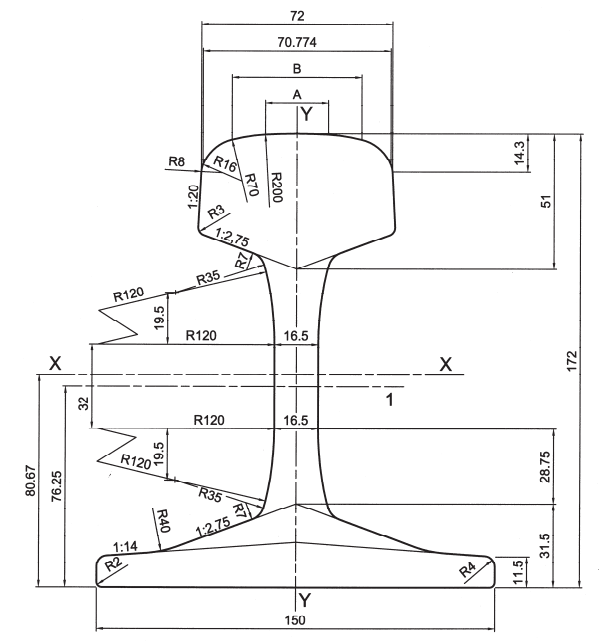
\includegraphics[width=0.6\textwidth]{60E2}
  \caption{Profil kolejnice 60E2~\cite{csn1}}
  \label{fig:60E2}
  
\end{figure}

Tady je text po obrázku...

\chapter{Ukázka vložení tabulky}
\label{chap:uvt}

Tady je text před tabulkou...

\begin{table}[h!]
	\centering
	\caption{Oblačnost a průměrný teplotní rozdíl}
	\label{tab:otr}
	\begin{tabular}{|c|c|}
		\hline
		\rowcolor{green!50}
		\textbf{Oblačnost} & \textbf{Průměrný teplotní rozdíl [°C]} \\
		\hline
		\rowcolor{yellow!40}
		100 \% & 4.769 \\
		\hline
		\rowcolor{yellow!40}
		90 \% & 7.769 \\
		\hline
		\rowcolor{yellow!40}
		80 \% & 8.357 \\
		\hline
		\rowcolor{yellow!40}
		70 \% & 9.533 \\
		\hline
		\rowcolor{yellow!40}
		60 \% & 9.838 \\
		\hline
		\rowcolor{yellow!40}
		50 \% & 10.769 \\
		\hline
		\rowcolor{yellow!40}
		40 \% & 11.082 \\
		\hline
		\rowcolor{yellow!40}
		30 \% & 10.767 \\
		\hline
		\rowcolor{yellow!40}
		20 \% & 13.900 \\
		\hline
		\rowcolor{yellow!40}
		10 \% & 11.860 \\
		\hline
		\rowcolor{yellow!40}
		0 \% & 11.325 \\
		\hline
	\end{tabular}
\end{table}

Tady je text po tabulce...

\chapter{Závěr}

Tady je závěr...

\nocite{*}																						% zahrne literaturu necitovanou v textu práce ve výpise literatury
\printbibliography[title={Použitá literatura},heading=bibnumbered]								% výpis literatury

\chapter{Přílohy}

\end{document}